% Overview Slide
\begin{frame}

\begin{itemize}
    \item \emph{\color{UOYellow}Flexible Neural Machine Translation Architecture
        Combination}
    \begin{itemize}
    \emph{\color{UOYellow}
        \item Neural Machine Translation (NMT)
        \item Architecture Definition Language (ADL)
        \item Layer Definitions
        \item Standard Architectures
    }
    \end{itemize}
    \item Related Work
    \item Experiments
    \item Conclusion
\end{itemize}

\end{frame}

% 2.1
\begin{frame}
\frametitle{Neural Machine Translation (NMT)}

\begin{itemize} 
    \item NMT is a sequence to sequence prediction task 
\end{itemize}
\[
    X \mapsto Y
\]
\[
    p(y_t | Y_{1:t-1}, X; \boldsymbol{\theta}) = \text{softmax}(\boldsymbol{W}_o
            \boldsymbol{z}^L + \boldsymbol{b}_o)
\]

\begin{itemize}
    \item $\boldsymbol{W}_o$ projects a model dependent hidden vector
    $\boldsymbol{z}^L$ of the L$^\text{th}$ decoder layer to the dimension of
    the target vocabulary $\boldsymbol{V}_{trg}$
    \item Training minimizes cross-entropy loss
\end{itemize}

\end{frame}

%2.2
\begin{frame}
\frametitle{Architecture Definition Language (ADL)}
    \begin{columns}
        \begin{column}{0.55\paperwidth}
        \begin{itemize}
            \item ADL is a language used to describe network structures.
            \item This language lets us discuss a NMT in an easy to understand manner.
            \item E.G. $pos \rightarrow repeat(n,res(cnn(glu) \rightarrow dropout))$ 
            \begin{itemize}
                \item Positional encoding $\rightarrow$ residual CNN with gated linear
                units $\rightarrow$ dropout
            \end{itemize}
        \end{itemize}
    \end{column}
        \begin{column}{0.39\paperwidth}
            \vspace{-1cm}
            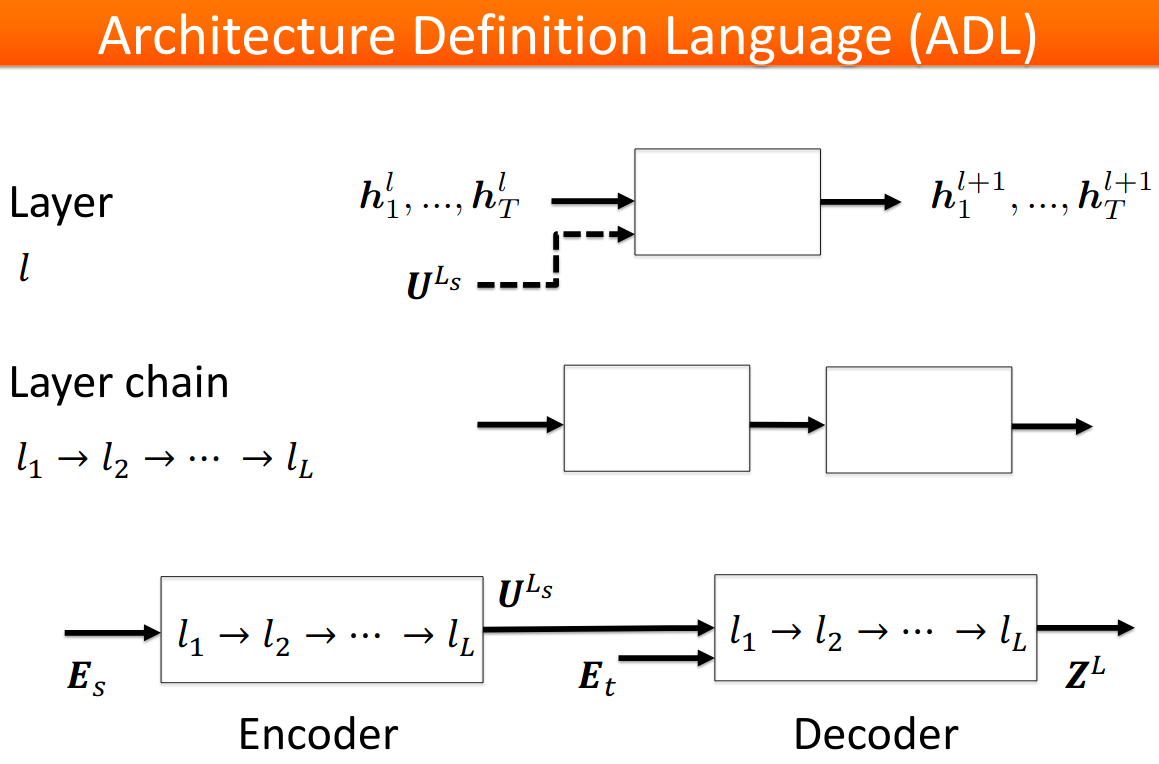
\includegraphics[width=\textwidth]{ADL.png}\\
            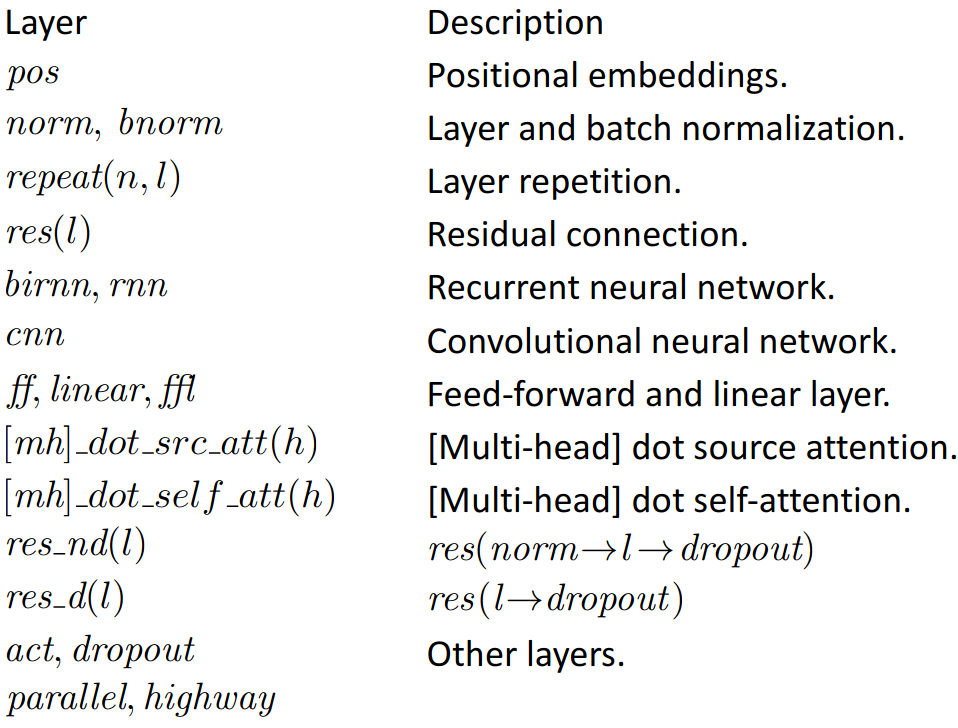
\includegraphics[width=\textwidth]{ADL_def.png}
        \end{column}
\end{columns}
\end{frame}
